\section{Inverse Reinforcement Learning}

\begin{frame}
	\frametitle{IRL Problem Definition}
	
	\Large
	
	\begin{equation*}
		\begin{array}{ll}
			\max \sum\limits_{i=1}^N \min\limits_{a \in \mathbf{A}} \Big
			\{ \big [ \mathbf{P}_{a_*}(i) - \mathbf{P}_a(i) \big ] ( \mathbf{I} - \gamma
			\mathbf{P}_{a_*})^{-1} \mathbf{R} \Big \} - \lambda \| \mathbf{R} \|_1 \\ \\
			s.t. \\ \;\;\;\;
			\left \{
				\begin{array}{ll}
					(\mathbf{P}_{a_*} - \mathbf{P}_a)(\mathbf{I} - \gamma
					\mathbf{P}_{a_*})^{-1} \, \mathbf{R} \succeq 0 \;\,\,\,\, \forall \, a \in
					\mathbf{A} \\ \\
					| \mathbf{R}_i | \leq R_{max} \;\;\;\;\;\;\;\;\;\;\;\;\;\;\;\;\;\;\;\;\;\
					\;\;\;\;\;\;\;\;\,\,\,\,\, i \, \in \{ 1, \ldots, N \}
				\end{array}
			\right.
			\vspace{0.2cm}
		\end{array}
	\end{equation*}
\end{frame}

\begin{frame}
	\frametitle{Toward a Linear Program Definition}
	
	\Large
	
	\vspace{0.4cm}
	
	The \emph{non-linear} 1-norm operator $ \| \mathbf{R} \|_1 $ of the original problem should
	be linearized by adding two more variables $ r_i^+ $ and $ r_i^- $ for every $ r_i $
	variable with $ i \, \in \{ 1, \ldots, N \} $.
	
	\vspace{0.8cm}
	
	The \emph{non-linear} operator $ \min\limits_{a \in \mathbf{A}} $, instead, should be
	linearized by introducing $ N $ new variables $ x_i $ where $ i \, \in \{ 1, \ldots, N \} $
\end{frame}

\begin{frame}
	\frametitle{IRL Linear Program Definition}
	
	\Large
	
	\vspace{-0.3cm}
	
	\begin{equation*}
		\begin{array}{ll}
			\min \sum\limits_{i=1}^N -x_i + \lambda (r_i^+ - r_i^-)
			\vspace{-0.35cm} \\ \\
			s.t. \\ \;\;\;\;
			\left \{
				\begin{array}{ll}
					x_i \leq (\mathbf{P}_{a_*} - \mathbf{P}_a)(\mathbf{I} - \gamma
					\mathbf{P}_{a_*})^{-1} \mathbf{R} \\
					\vspace{-0.25cm} \\
					\;\;\;\;\;\;\;\;\;\,\,\;\;\;\;\;\;\;\;\;\;\;\;\;\;\;\;\;\;\;\;\;\;\;\;\;\;
					\;\;\; \forall \, a \in \mathbf{A}, \; i \in \{ 1, \ldots, N \}
					\vspace{-0.25cm}\\ \\
					x_i \geq 0 \;\;\;\;\;\;\,\,\,\,\;\;\;\,\,\,\,\,\;\,\,\,\,\,\,\,\;\;\;\;\;
					\;\;\;\;\;\;\;\;\;\;\;\;\;\,\,\;\,\,\,\,\,\, i \, \in \{ 1, \ldots, N \}
					\vspace{-0.25cm} \\ \\
					r_i = r_i^+ + r_i^- \;\,\,\,\,\,\;\,\,\,\,\,\,\,\;\;\;\;\;
					\;\;\;\;\;\;\;\;\;\;\;\;\,\,\,\,\,\,\,\,\,\,\,\,\, i \, \in \{ 1, \ldots, N \}
					\vspace{-0.25cm}
					\\ \\
					| \mathbf{R}_i | \leq R_{max} \;\;\;\;\;\;\;\;\;\;\;\,\,\,\,\;\;\
					\;\;\;\;\;\;\;\;\;\;\;\,\,\;\;\;\,\,\,\,\,\, i \, \in \{ 1, \ldots, N \}
				\end{array}
			\right.
			\vspace{0.2cm}
		\end{array}
	\end{equation*}
\end{frame}

\begin{frame}
	\frametitle{A Simple Example}
	
	\vspace{0.1cm}
	
	\begin{center}
		\begin{tikzpicture}
			\node at (0,0) [draw=white,ultra thick,inner sep=0pt]
			{
				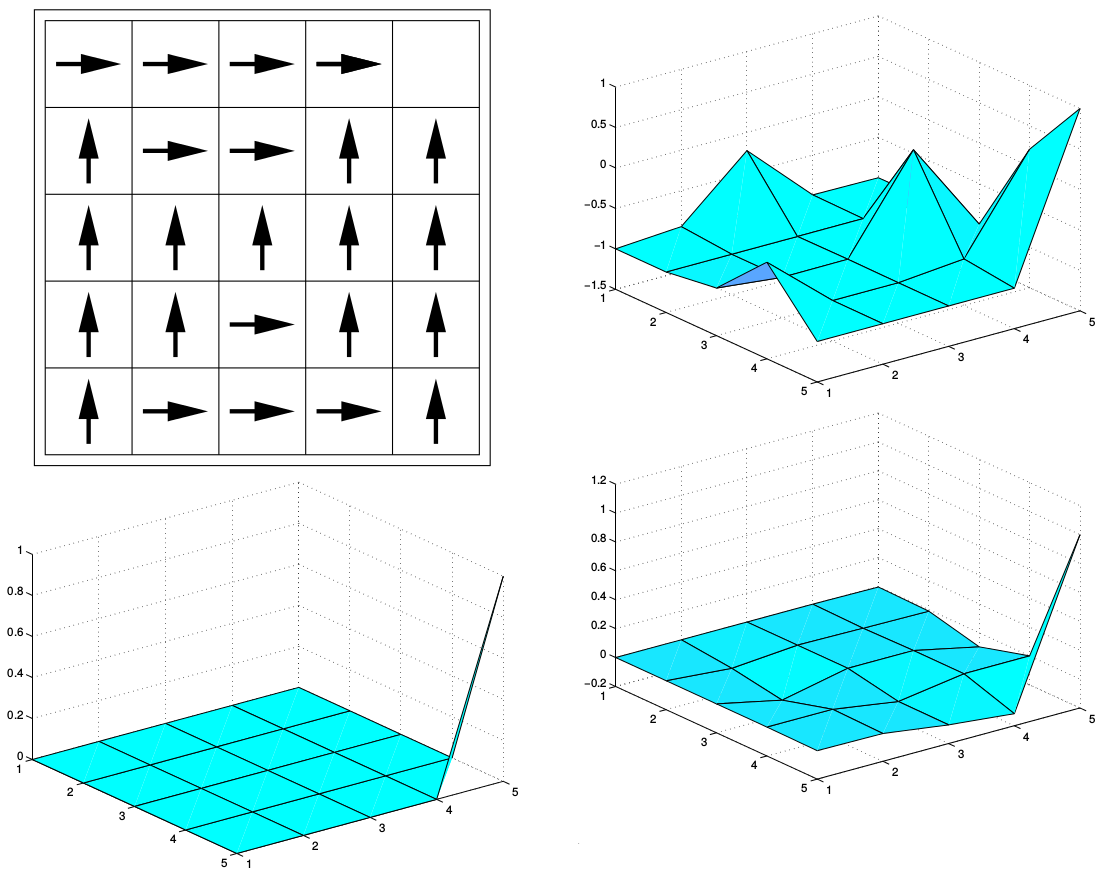
\includegraphics[scale=0.23]{Figures/GridExample.png}
			};
		\end{tikzpicture}
	\end{center}
\end{frame}


	
	
	

